\documentclass[9pt]{pnas-new}
% Use the lineno option to display guide line numbers if required.
% Note that the use of elements such as single-column equations
% may affect the guide line number alignment. 

\RequirePackage[english,slovene]{babel} % when writing in slovene
%\RequirePackage[slovene,english]{babel} % when writing in english

\templatetype{pnasresearcharticle} % Choose template 
% {pnasresearcharticle} = Template for a two-column research article
% {pnasmathematics} = Template for a one-column mathematics article
% {pnasinvited} = Template for a PNAS invited submission

% \selectlanguage{slovene}
% \etal{in sod.} % comment out when writing in english
% \renewcommand{\Authands}{ in } % comment out when writing in english
% \renewcommand{\Authand}{ in } % comment out when writing in english

\newcommand{\set}[1]{\ensuremath{\mathbf{#1}}}
\renewcommand{\vec}[1]{\ensuremath{\mathbf{#1}}}
\newcommand{\uvec}[1]{\ensuremath{\hat{\vec{#1}}}}
\newcommand{\const}[1]{{\ensuremath{\kappa_\mathrm{#1}}}} 

\newcommand{\num}[1]{#1}

\graphicspath{{./fig/}}

\title{Collective Behaviour Report 2 : Simulating Schooling Fish Feeding Behaviour}

% Use letters for affiliations, numbers to show equal authorship (if applicable) and to indicate the corresponding author
\author{Melinda Fabien}
\author{Sarah Gay}
\author{Ana Gelez}
\author{Alina Sereda}

\affil{Collective behaviour course research seminar report} 

% Please give the surname of the lead author for the running footer
\leadauthor{Fabien} 

\selectlanguage{english}


% Please include corresponding author, author contribution and author declaration information
%\authorcontributions{Please provide details of author contributions here.}
%\authordeclaration{Please declare any conflict of interest here.}
%\equalauthors{\textsuperscript{1}A.O.(Author One) and A.T. (Author Two) contributed equally to this work (remove if not applicable).}
%\correspondingauthor{\textsuperscript{2}To whom correspondence should be addressed. E-mail: author.two\@email.com}

% Keywords are not mandatory, but authors are strongly encouraged to provide them. If provided, please include two to five keywords, separated by the pipe symbol, e.g:
\keywords{Boids| Fishes | Aquaculture | 3D Engine} 

\begin{abstract}
In this paper, we introduce a simulation model depicting the collective behavior of a school of fish within a tank. We are interested in modeling the behavior of fishes in order to identify the optimal way to feed them. We describe our simulation model and how we implemented it.Then,we review the results and explore ways to enhance our simulation by considering more parameters, aiming for increased realism.
\end{abstract}

\dates{\textbf{\today}}
\program{BM-RI}
\vol{2018/19}
\no{CB:G1} % group ID
%\fraca{FRIteza/201516.130}

\begin{document}

% Optional adjustment to line up main text (after abstract) of first page with line numbers, when using both lineno and twocolumn options.
% You should only change this length when you've finalised the article contents.
\verticaladjustment{-2pt}

\maketitle
\thispagestyle{firststyle}
\ifthenelse{\boolean{shortarticle}}{\ifthenelse{\boolean{singlecolumn}}{\abscontentformatted}{\abscontent}}{}

% If your first paragraph (i.e. with the \dropcap) contains a list environment (quote, quotation, theorem, definition, enumerate, itemize...), the line after the list may have some extra indentation. If this is the case, add \parshape=0 to the end of the list environment.
\dropcap{E}stimating optimal living conditions for fish in aquaculture can be challenging due to the expense, time, and potential harm to the fish involved in traditional testing methods. In the referenced paper \cite{article}, the authors proposed various testing methods for optimizing the distribution system in a simulated fish tank environment. The aim is to optimize the feeding distribution system in aquaculture, thereby improving management and creating conditions for accelerated fish growth, all while saving time and resources. 

Although this simulation provides significant results that can be used, it is also limited since it only applies to the rainbow trout species.  Furthermore, it neglects considerations of other environmental variables, such as the possibility of fish mortality resulting from malnutrition. 

The goal of our project is to enhance this highly promising simulation by incorporating additional features.The initial step is to reproduce this simulation using our own means. After obtaining the first results, we will discuss to identify relevant and feasible extensions. If we find them beneficial, they will be integrated into our model.

\section*{Methods}

For this step, we finished to reach the original simulation state. We are gaining in confidence on Godot and corrected ourselves on a few inaccuracies we had.

\subsection{Implementation model based}

The simulation provided by the article is divided into two main parts: Feeding and Growth. These two phases alternate continually until reaching a certain limit (either a specified number of days or a predefined time) or reaching a capacity limit in the aquarium.

\subsubsection{Feeding simulation}

In this section, we focus on the way the fish are fed. In the initial iterations, we chose the default weight for fish of 38.53g. This value was derived from studies conducted in the following study \cite{morales1994effects}, specifically for rainbow trout. However, it is fish-specific and would need adaptation if we intend to extend this experiment to other fish species.

The model individually evaluates the amount of food ingested by each fish, taking into account the fish's size and mass.
Whenever a fish comes into contact with a pellet, the cumulative count of pellets it has encountered increases. Then, we used this count to calculate the `feed\_intake\_weight`, which involves multiplying the weight of a pellet with the number of pellets ingested by the fish during this phase.

To calculate the amount of food that need to be given, we proceed as follows : one food pellet weights 0.065g so for this second milestone, we don't drop one pellet at a time anymore but, following the original simulation, the equivalent in pellets of 1.86\% of the total mass of fishes. To simplify : all the fishes weights are added together, then we calculate 1.86\% of this mass and give the equivalent in pellets. Since 1.86\% is a pretty low rate, we will have to think about modify it in order for fishes to grow faster.

\subsubsection{Growth simulation}

Following the Feeding Simulation phase, we enter the Growth phase. Depending on the quantity of food ingested by the fish in the previous phase, it will experience varying degrees of growth. To accurately calculate this, we employ the Feed Conversion Efficiency (FCE).

The choice of FCE being set to 1.0 is deliberate. A value of 1.0 for FCE implies that all the ingested food contributes directly to the fish's body mass gain. This simplification is used to maintain straightforward relationship between feed intake and growth, especially since we don't have more information about their metabolic system. 

After the body mass was updated, total length was calculated from the following allometric equation:

\[W_n^i = (a \times TL_n^i)^b\] 

where \(TL_n^i\) is the total length of the i-th individual on the n-th day and a and b are coefficients of allometry; here, a was 0.0209 and b was 2.843, respectively

It is equally important to prevent excessive daily growth in fish size. To address this, we implement a safeguard by establishing a maximum size the fish can achieve in a single day, capped at 4\% of the fish's body mass.

\subsubsection{Movement model of the fish}

Each fish adheres to the following movement model:

\[W_n^i a_{t+\Delta t} = F_t\]
\[v_{t+\Delta t} = v_t +  a_{t+\Delta t}*\Delta t\]
\[x_{t+\Delta t} = x_t + v_{t+\Delta t} *\Delta t\]


Depending on whether there is food in the aquaculture tank or not, the fish's movement model will change.

\begin{figure}[h]
    \centering
    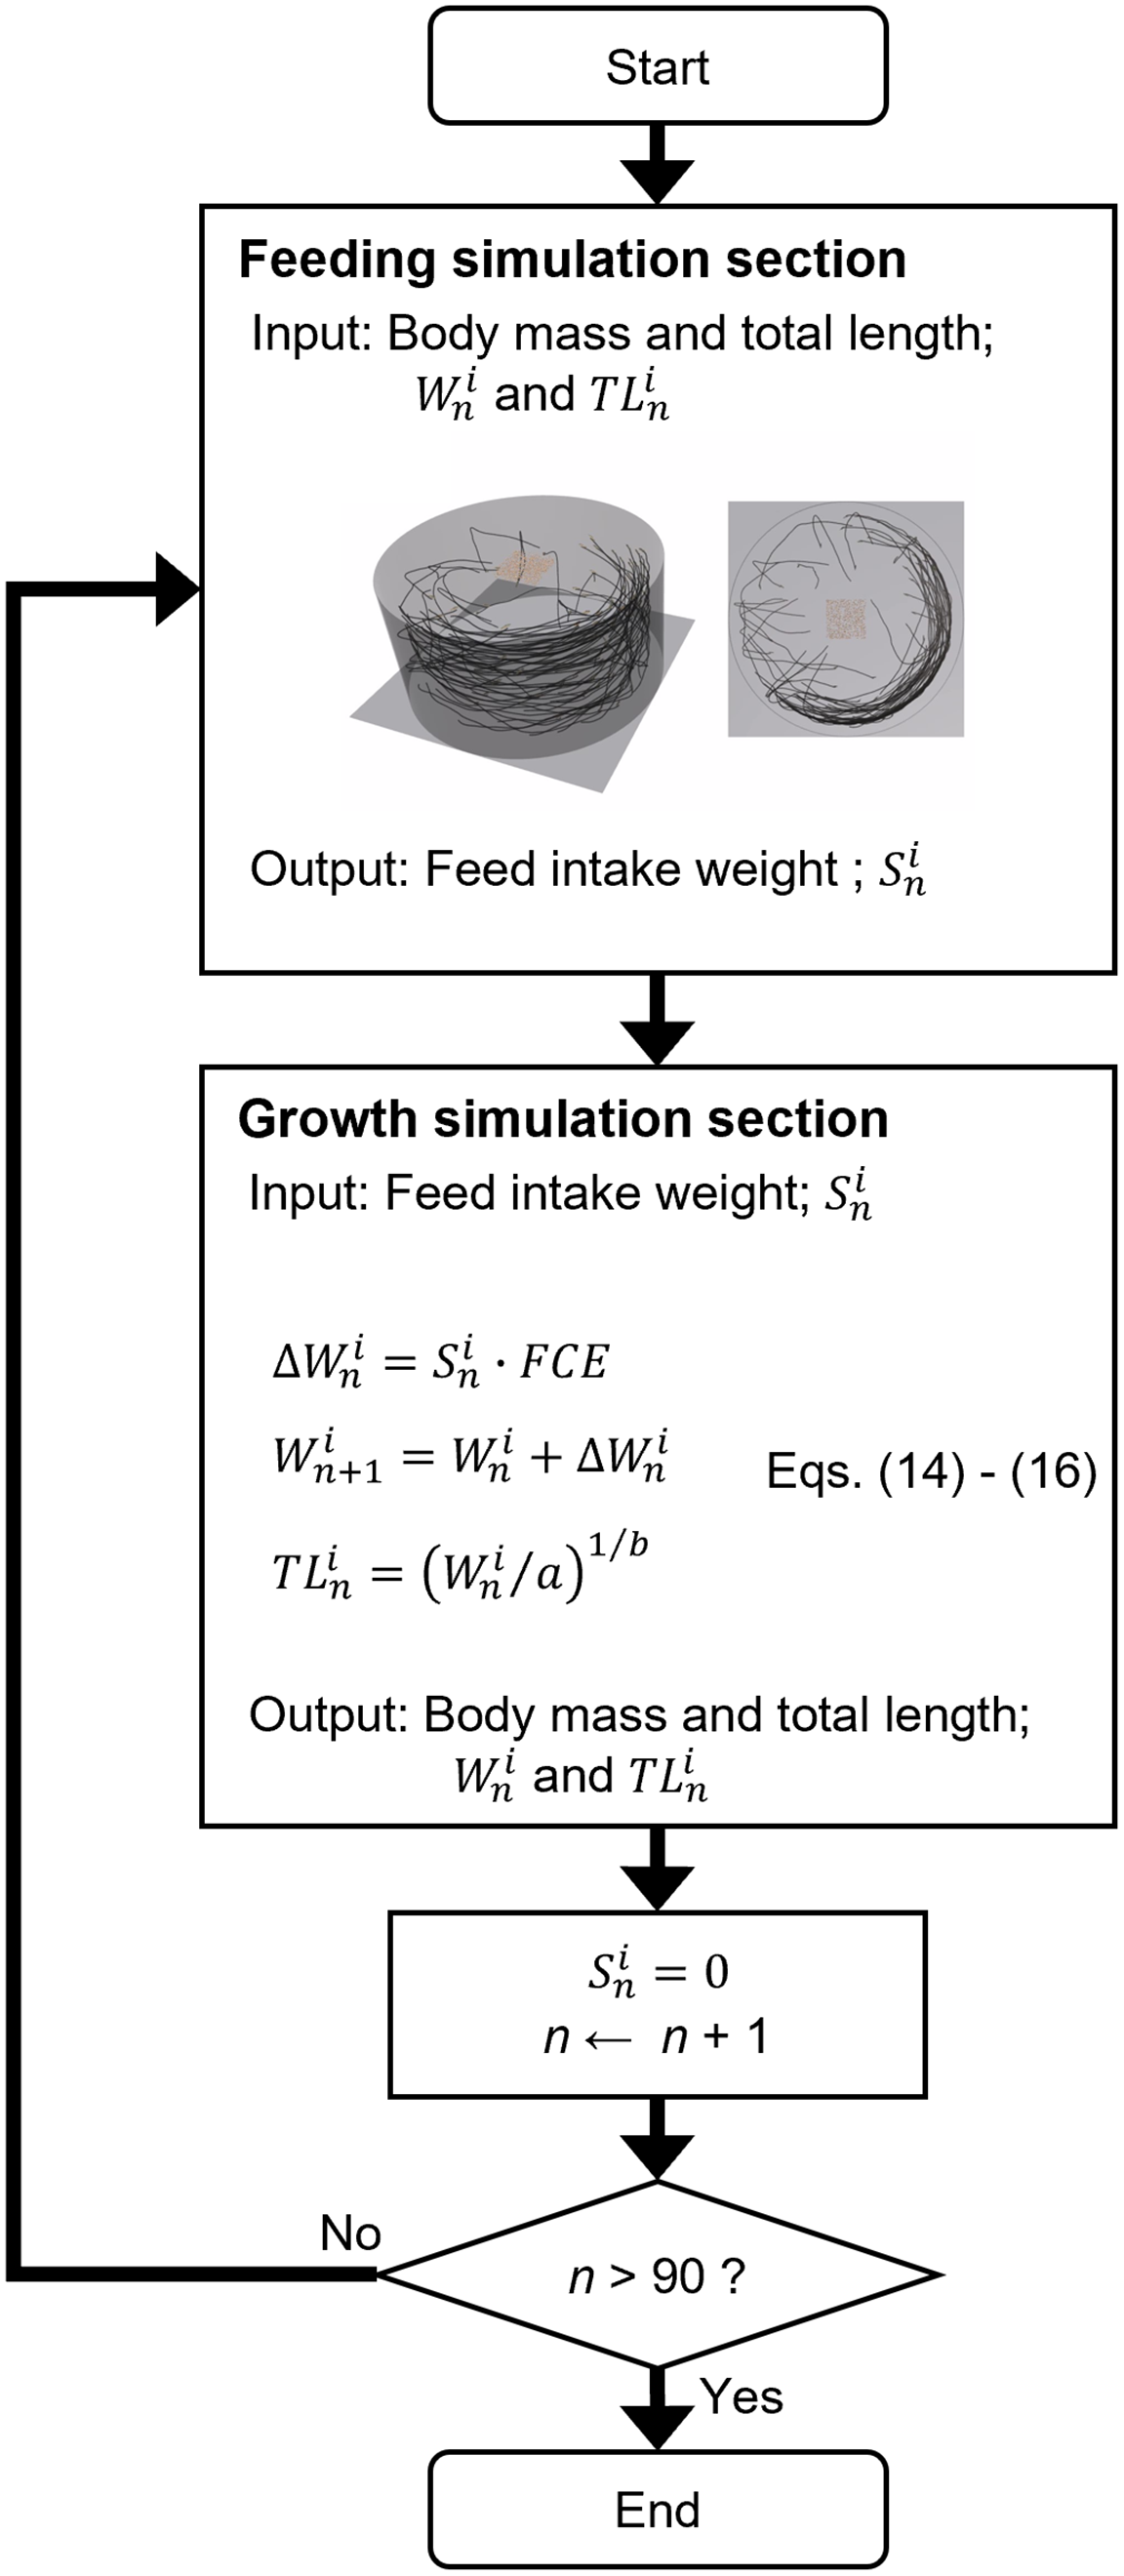
\includegraphics[width=0.3\linewidth]{figure3.PNG}
    \caption{Simulation Model}
    \label{fig:figure1}
\end{figure}

During the feeding phase (see Figure \ref{fig:figure1}), the fish will move more quickly towards the food. The vector v5 \(TL_n^i\) corresponding to vector in our model, transitions from 0 to 3 if the fish is not satiated (i.e., it has not exceeded the maximum size it can gain in a day). The speed coefficients used in the movement equations are also adjusted to change from 1.5 to 7. 

In the simulation, each fish has a limited field of view that influences its movement based on the presence or absence of boundaries within this range.The size of the field of view is twice the total length of the fish. There is also a dead space directly behind the fish where visibility is compromised  (see Figure \ref{fig:Field of view}): .However, the fish's ability to detect food remains unaffected, as individuals can sense the food regardless of their field of view. 


\begin{figure}[h]
    \centering
    \begin{minipage}[b]{0.5\linewidth}
        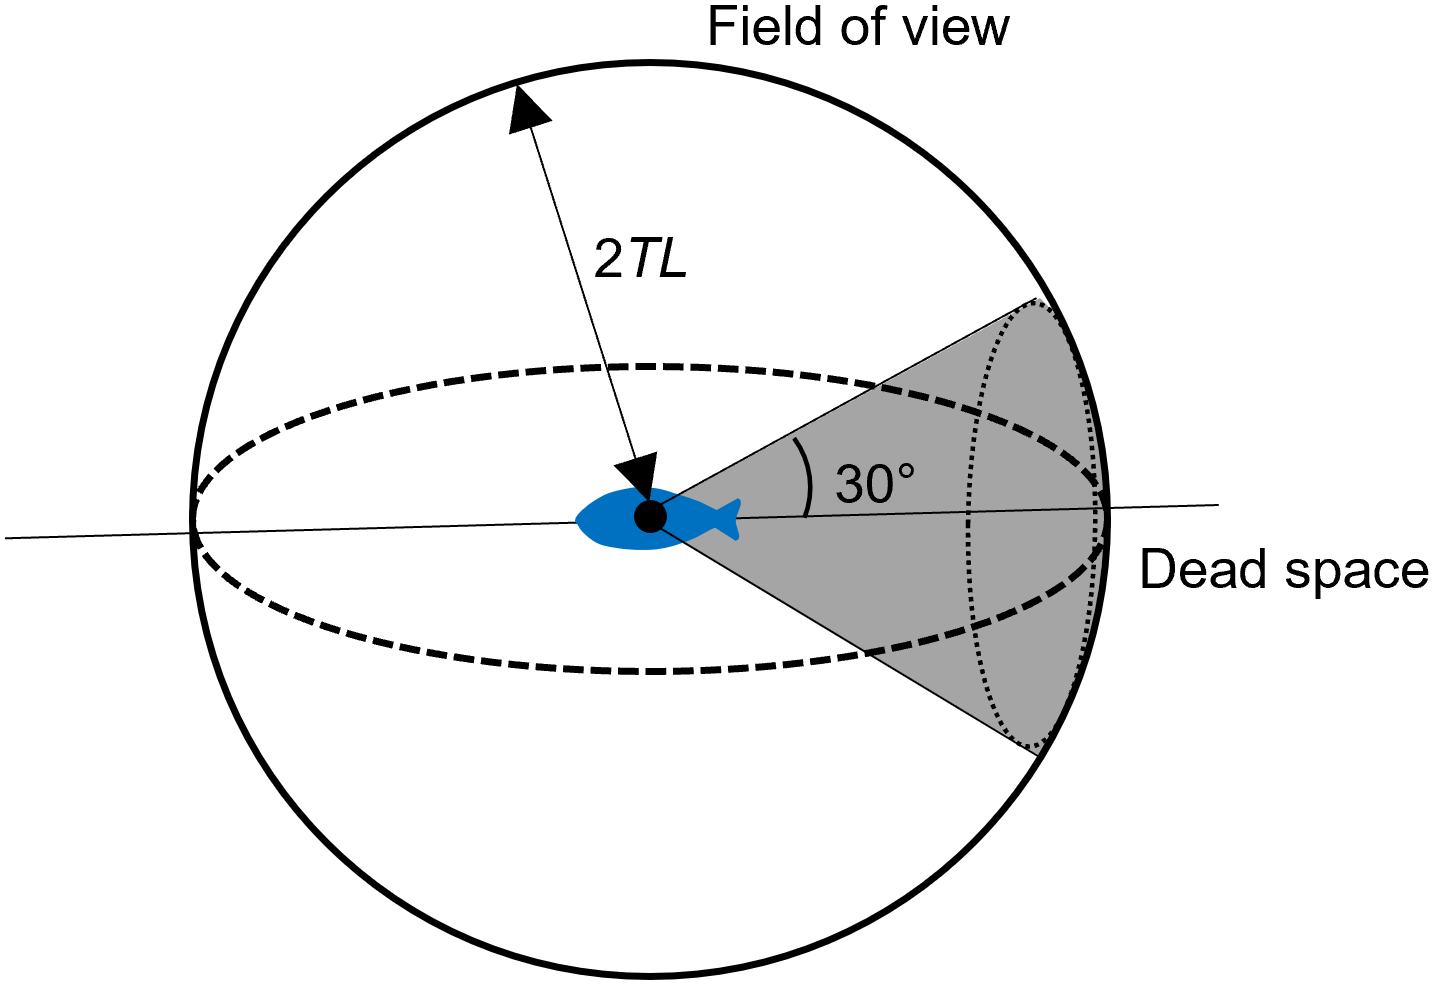
\includegraphics[width=\textwidth]{fig/field_of_view.PNG}
        \caption{field of view of a fish}
        \label{fig:Field of view}
    \end{minipage}
\end{figure}


The collective behavior of individuals within the system is defined by distinct rules. \textbf{Separation} prompts them to maintain distance from their nearest peers, avoiding congestion. Simultaneously, the principle of \textbf{Alignment} encourages them to move harmoniously in the same direction, fostering coordination. \textbf{Cohesion} drives them to converge toward the center of their companions, enhancing social proximity. When \textbf{Approaching feed}, individuals are drawn towards food sources, ensuring efficient feeding. The instinct of \textbf{avoiding boundaries} prevents them from getting too close to edges, offering protection. Lastly, \textbf{Random movement} injects spontaneity, contributing to the diversity of group dynamics. These rules collectively shape the dynamic interactions, yielding a nuanced and adaptive system.

To see the details of the equation, refer to this article \cite{article}

\subsection{Setup and visualization of the fish}
We decided to both simulate and visualize the fish behaviour with Godot Engine which is a tool quite similar to Unity. It uses its particular programming language, GDScript, which is Python inspired. For the simulation, we used two classes : Food and Fish. The tank and its details is created in the main so the bulk of the function is in the two first classes.
\begin{itemize}
    \item \textbf{Food} : This one is the simplest and set the weight and the movement of the pellet once dropped into the tank
    \item \textbf{Fish} :  This class takes care of simulating the size and behaviour of fish but also the two phases explained above. It manages the modification in behaviour when food is detected by fish, the growth when eating food and the collective behaviour of the school as mentioned.
\end{itemize}   

\section{Results}

Currently, we have successfully implemented the food distribution system. To generate food, a simple click on the screen is sufficient, triggering the appearance of the food. Additionally, we have established the tank environment where the fish can swim and have implemented the underlying logic of the swimming force.

\begin{figure}[h]
    \centering
    \begin{minipage}[b]{0.45\linewidth}
        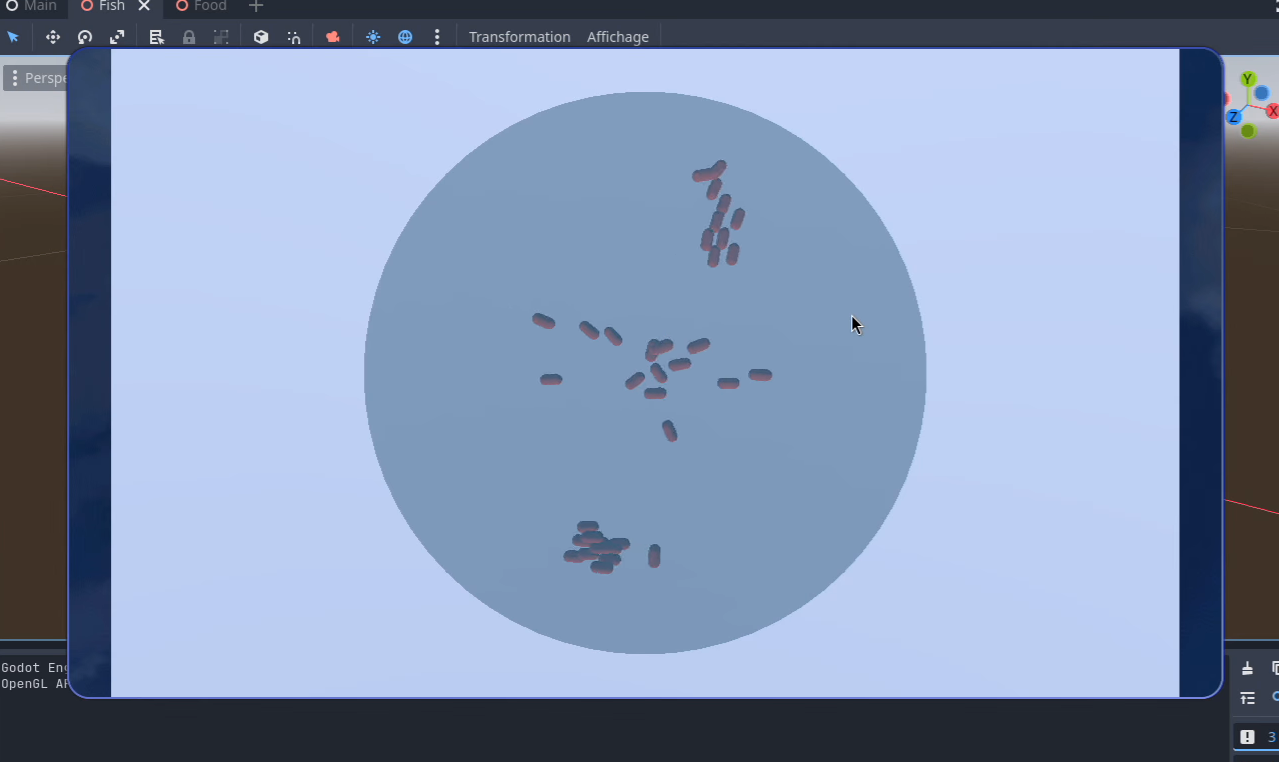
\includegraphics[width=\textwidth]{Capture.PNG}
        \caption{Top View of the simulation}
        \label{fig:Top view tankl}
    \end{minipage}
    \hspace{0.5cm}
    \begin{minipage}[b]{0.45\linewidth}
        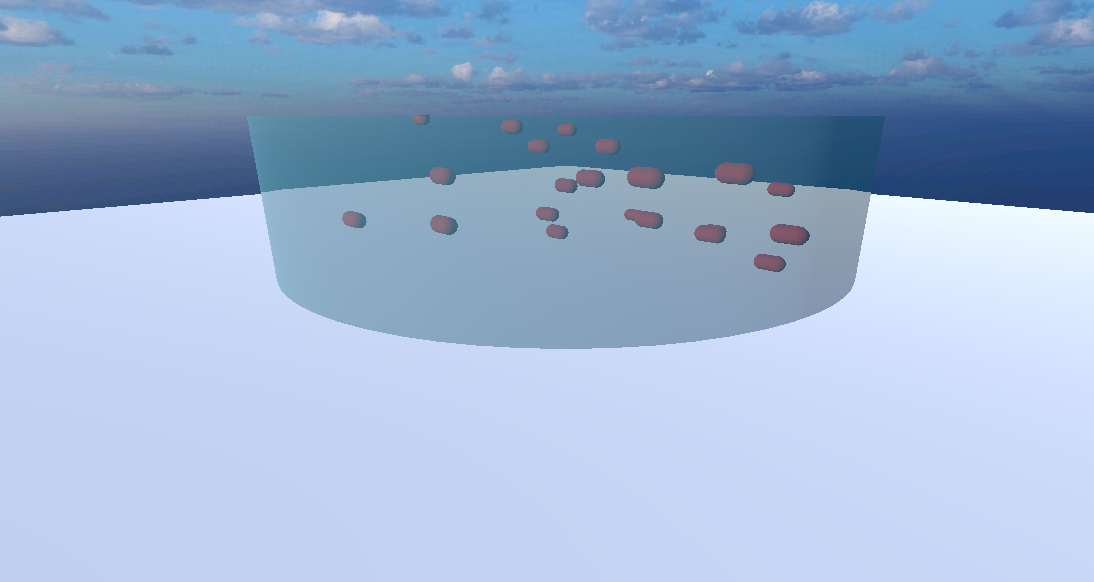
\includegraphics[width=\textwidth]{poisson2.png}
        \caption{View of the simulation}
        \label{fig: basic view tankl}
    \end{minipage}
\end{figure}

We've implemented behavioural aspects into the fish schooling movement, including food attraction. When there's food in the tank, the fish move faster. Additionally, certain fish can form groups and behave like it, while also avoiding boundaries.

We use a text file to collect important data, noting the number of fish and their sizes at the end of the simulation. This file serves as a dataset for comparing the effectiveness of different distribution systems. We calculate mean values for each system to measure of their overall performance.   


\section{Discussion}
\subsection{What are the future tasks ?}
For now we have implemented the simulation presented in the paper. Thanks to our work, we have a better idea of the evaluation criteria for the simulations to be done. Indeed, we will have to try several values for our parameters like the pellet's weight or the feed conversion efficiency. This part would be useful to compare our results with those of the paper and have a real checkpoint regarding our project.


\begin{figure}
    \centering
    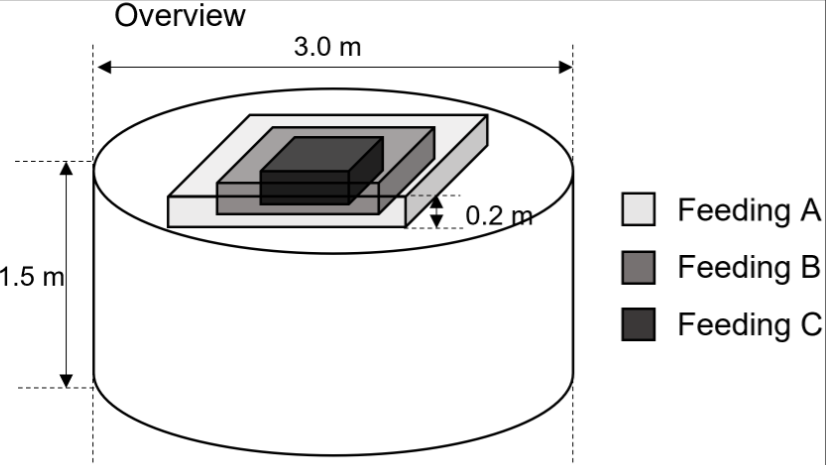
\includegraphics[width=0.3\linewidth]{fig5.png}
    \caption{Simulation field}
    \label{fig:enter-label}
\end{figure}

After this step, we will first finish the improvement of fish aesthetics for them to look like actual fishes because with the model we found, their size is increasing too fast. Then we will add further details such as integrate a pellet counter to track fish food consumption. Additionally, we will automate the food distribution system for simplified management. We will introduce a limiting feature, either in terms of time or the number of fish, for precise control over simulation parameters.

\subsection{What kind of extensions can be added?}
Since we currently have implemented the original simulation, we are planning to hold a meeting soon to choose which extensions will be done. For the moment, we have a better idea of the feasibility of each one of them. Here's what we've already thought of :

\small\subsubsection*{Feeding Parameters}
\begin{itemize}
    \item Different feeding areas: line shape, cross shape, multiple points around the tank, increasing or reducing pellet weight. Different distribution methods can be useful to find the best way to feed fish.
\end{itemize}

\small\subsubsection*{Adding New Parameters Defining Fish Life}
\begin{itemize}
    \item Add realism to the model by:
        \begin{itemize}
            \item Implementing death by malnutrition after a certain time.
            \item Implementing death by asphyxiation by managing oxygen in the tank. It's crucial in aquaculture since it's one of the leading causes of fish mortality
        \end{itemize}
    \item Consider other types of fish used in aquaculture. A paper providing information about Atlantic salmon \cite{handeland2008effect} can be used to understand how a different species behaves under similar conditions.
\end{itemize}




\section{Conclusion }
To summarize what has been done, we now have nearly reproduced the model proposed in the original paper. We have also planned the next steps which are to automate the food dropping and the population of fish management and to discuss the extensions that will be implemented in order to make the simulation more realistic.

\section{Contributions}
\begin{itemize}
    \item \textbf{Ana:} Implemented the \verb Fish  class, defining the primary behavior of the fish +  writing of the reports (abstract section) + polishing of the English language.

    \item \textbf{Sarah:} Implemented the food distribution system + writing the report (Discussion, Results, and Conclusion sections).

    \item \textbf{Mélinda:} Enhanced the aesthetic aspects of the fish and made minor corrections about fish behaviour + writing the reports (focusing on the Introduction and Methods section)

    \item \textbf{Alina:} Working on the report + final verification of the report + grammar check
    
\end{itemize}

    

\begin{multicols}{2}
\section*{\bibname}
% Bibliography
\bibliography{./bib/bibliography}
\end{multicols}

\end{document}